\documentclass[openany]{report}
\usepackage{lmodern}
\usepackage{amssymb,amsmath}
\usepackage{ifxetex,ifluatex}
\usepackage{fixltx2e} % provides \textsubscript
\ifnum 0\ifxetex 1\fi\ifluatex 1\fi=0 % if pdftex
  \usepackage[T1]{fontenc}
  \usepackage[utf8]{inputenc}
\else % if luatex or xelatex
  \ifxetex
    \usepackage{mathspec}
  \else
    \usepackage{fontspec}
  \fi
  \defaultfontfeatures{Ligatures=TeX,Scale=MatchLowercase}
\fi
% use upquote if available, for straight quotes in verbatim environments
\IfFileExists{upquote.sty}{\usepackage{upquote}}{}
% use microtype if available
\IfFileExists{microtype.sty}{%
\usepackage{microtype}
\UseMicrotypeSet[protrusion]{basicmath} % disable protrusion for tt fonts
}{}
\usepackage{hyperref}
\hypersetup{unicode=true,
            pdftitle={Systems Pathology: Muscle System},
            pdfauthor={Russell Fraser},
            pdfborder={0 0 0},
            breaklinks=true}
\urlstyle{same}  % don't use monospace font for urls
\usepackage{natbib}
\bibliographystyle{apalike}
\usepackage{longtable,booktabs}
\usepackage{graphicx,grffile}
\makeatletter
\def\maxwidth{\ifdim\Gin@nat@width>\linewidth\linewidth\else\Gin@nat@width\fi}
\def\maxheight{\ifdim\Gin@nat@height>\textheight\textheight\else\Gin@nat@height\fi}
\makeatother
% Scale images if necessary, so that they will not overflow the page
% margins by default, and it is still possible to overwrite the defaults
% using explicit options in \includegraphics[width, height, ...]{}
\setkeys{Gin}{width=\maxwidth,height=\maxheight,keepaspectratio}
\IfFileExists{parskip.sty}{%
\usepackage{parskip}
}{% else
\setlength{\parindent}{0pt}
\setlength{\parskip}{6pt plus 2pt minus 1pt}
}
\setlength{\emergencystretch}{3em}  % prevent overfull lines
\providecommand{\tightlist}{%
  \setlength{\itemsep}{0pt}\setlength{\parskip}{0pt}}
\setcounter{secnumdepth}{5}
% Redefines (sub)paragraphs to behave more like sections
\ifx\paragraph\undefined\else
\let\oldparagraph\paragraph
\renewcommand{\paragraph}[1]{\oldparagraph{#1}\mbox{}}
\fi
\ifx\subparagraph\undefined\else
\let\oldsubparagraph\subparagraph
\renewcommand{\subparagraph}[1]{\oldsubparagraph{#1}\mbox{}}
\fi

%%% Use protect on footnotes to avoid problems with footnotes in titles
\let\rmarkdownfootnote\footnote%
\def\footnote{\protect\rmarkdownfootnote}

%%% Change title format to be more compact
\usepackage{titling}

% Create subtitle command for use in maketitle
\providecommand{\subtitle}[1]{
  \posttitle{
    \begin{center}\large#1\end{center}
    }
}

\setlength{\droptitle}{-2em}

  \title{Systems Pathology: Muscle System}
    \pretitle{\vspace{\droptitle}\centering\huge}
  \posttitle{\par}
    \author{Russell Fraser}
    \preauthor{\centering\large\emph}
  \postauthor{\par}
      \predate{\centering\large\emph}
  \postdate{\par}
    \date{2019-10-31}

\usepackage{booktabs}
\usepackage{booktabs}
\usepackage{longtable}
\usepackage{array}
\usepackage{multirow}
\usepackage{wrapfig}
\usepackage{float}
\usepackage{colortbl}
\usepackage{pdflscape}
\usepackage{tabu}
\usepackage{threeparttable}
\usepackage{threeparttablex}
\usepackage[normalem]{ulem}
\usepackage{makecell}
\usepackage{xcolor}

\begin{document}
\maketitle

{
\setcounter{tocdepth}{1}
\tableofcontents
}
\chapter*{About}\label{about}
\addcontentsline{toc}{chapter}{About}

These notes are a fairly comprehensive collection of information to
complement the lectures and labs delivered in VETM2210, Systems
Pathology I, on the topic of skeletal muscle. Although all of the
information is useful, certain areas will have been emphasized in
lecture, let the areas focussed on in lectures and lab guide your
studying. There are a few rare conditions that are not discussed in
these notes, and you are encouraged to read through the relevant
chapters in the textbooks recommended below.

The notes are available online at \url{http://russfraser.ca/muscle/}, as
a PDF on Moodle, and as an Epub (E-book format, suitable for a tablet or
e-reader). Please feel free to provide feedback, whether on content,
style, or typos!

\subsection*{Contact me}\label{contact-me}
\addcontentsline{toc}{subsection}{Contact me}

Please don't hesitate to get in touch if you have any questions.

\begin{itemize}
\tightlist
\item
  Phone: 902-620-5183
\item
  E-mail: \href{mailto:rufraser@upei.ca}{\nolinkurl{rufraser@upei.ca}}
\item
  Office: 414N, Dept. of Pathology and Microbiology
\end{itemize}

\section*{Reference material}\label{reference-material}
\addcontentsline{toc}{section}{Reference material}

\begin{itemize}
\tightlist
\item
  Zachary, J. F., \& McGavin, M. D. (2016). Pathologic Basis of
  Veterinary Disease Expert Consult. Elsevier Health Sciences.
\item
  Maxie, G. (2015). Jubb, Kennedy \& Palmer's Pathology of Domestic
  Animals-E-Book (Vol. 1). Elsevier Health Sciences.
\end{itemize}

\section*{Acknowledgements}\label{acknowledgements}
\addcontentsline{toc}{section}{Acknowledgements}

These lecture notes were prepared in R \citep{R-base} using the bookdown
\citep{xie2015}, knitr \citep{R-knitr}, and Rmarkdown
\citep{R-rmarkdown} packages. Source material was taken from
\citet{zachary2016pathologic} and \citet{maxie2015jubb}. I gratefully
acknoweldge the prior course notes from Dr.~Paul Hanna. Images are
attributed throughout the text; unattributed images are either mine or
were found in the public domain.

\chapter{Introduction}\label{intro}

\hypertarget{the-anatomy-of-muscle}{\section{The anatomy of
muscle}\label{the-anatomy-of-muscle}}

The basic structural unit of muscle is the \textbf{myofiber}, which
represents a single, long, tubular cell (Figure
\ref{fig:muscle-structure}). Within each myofiber are many tightly
packed \textbf{myofibrils}, composed of actin and myosin filaments
(\textbf{myofilaments}), and which form the contractile machinery of the
muscle. It is the arrangment of myofibrils that form the striated
appearance of skeletal muscle that can be appreciated under light
microscopy (Figure \ref{fig:muscle-histo}). The cytoplasm of a myofiber
is known as the \textbf{sarcoplasm}, and the cell membrane is called the
\textbf{sarcolemma}. Each myofiber is surrounded by a small amount of
connective tissue called the \textbf{endomysium}. Multiple myofibers
form a \textbf{fasicle} that is surrounded by another layer of
connective tissue, the \textbf{perimysium}. Finally, multiple fasicles
group together to form a \textbf{muscle}, which is surrounded by the
epimysium.

\begin{figure}

{\centering 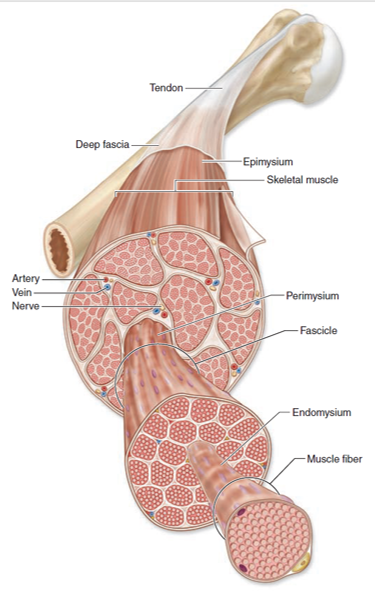
\includegraphics[width=0.4\linewidth]{images/muscle_structure} 

}

\caption{Structure and anatomy of muscle}\label{fig:muscle-structure}
\end{figure}

\begin{figure}

{\centering 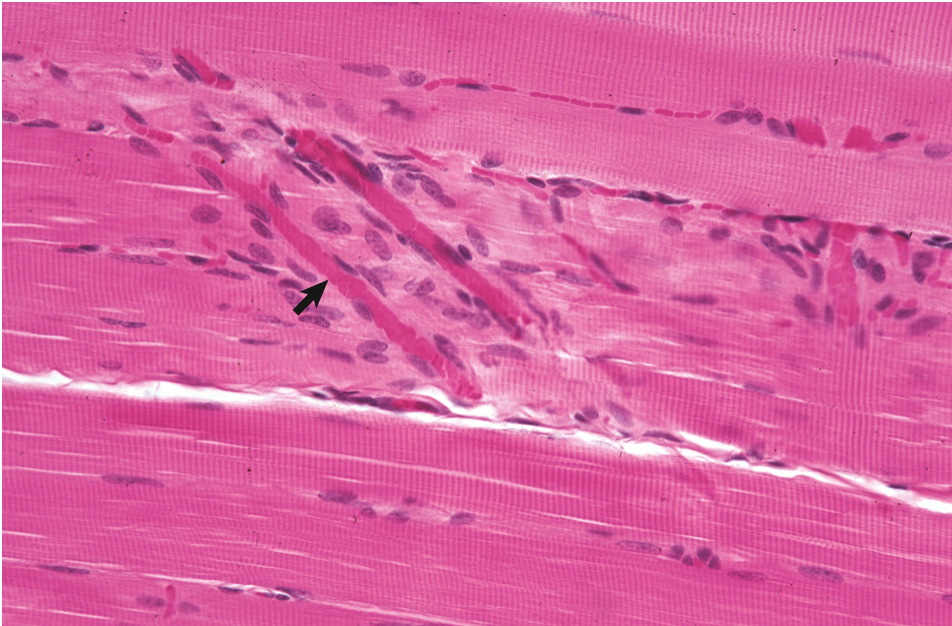
\includegraphics[width=0.5\linewidth]{images/muscle_histo} 

}

\caption{Normal skeletal muscle demonstrating striations. The arrow indicates a small capillary. Figure from Zachary and McGavin.}\label{fig:muscle-histo}
\end{figure}

Skeletal muscle is characteristically multinucleated: each myofiber has
hundreds of nuclei scattered along its length, almost always found along
the periphery of the cell. Each nucleus within a myofiber controls a
specific portion of the myofiber, and each nucleus acts independently.
Nuclei within muscle fibers are \emph{terminally differentiated},
meaning they can no longer divide, thus \textbf{limiting the capacity of
muscle for regeneration}. Having multiple nuclei within a cell provides
a distinct and somewhat unique benefit: localized damage, affecting a
small number of nuclei, will not necessarily kill the entire cell
(myofiber), and provides the myofiber with an opportunity to regenerate.
We will discuss muscle regeneration in more detail in the section on
\protect\hyperlink{necrosis-and-regeneration}{Necrosis and
regeneration}.

Closely associated with individual myofibers are \textbf{satellite
cells}. The nuclei of satellite cells are indistinguishable from
myofiber nuclei under light microscopy. Satellite cells are a type of
stem cell, and are important in muscle regeneration and repair.

Myofibers can be subclassified to reflect their function. The
classification is based on three physiologic properties:

\begin{enumerate}
\def\labelenumi{\arabic{enumi}.}
\tightlist
\item
  Rate of contraction (fast vs.~slow)
\item
  Rate of fatigue (fast vs.~slow)
\item
  Type of metabolism (oxidative, glycolytic, or mixed)
\end{enumerate}

Taking these characteristics into consideration leads to three subtypes:
Type 1, Type 2a, and Type 2b (Table \ref{tab:muscle-type}). Note that
muscles are rarely, if ever, composed of a single subtype: they are a
mixture of the different subtypes, though one type often predominates.

A basic review of the innervation of muscles is also worthwhile. Every
myofiber is innervated by a motor neuron, and each motor neuron
typically innervates multiple myofibers. The number of myofibers
innervated by a neuron is dependent on the need for fine control: only
1-4 myofibers of the occular muscles, for example, are innervated by a
single neuron, compared to the quadriceps where 150 or more myofibers
may be innervated by a single neuron.

\begin{table}[!h]

\caption{\label{tab:muscle-type}Properties of different myofiber types}
\centering
\begin{tabular}{l>{\raggedright\arraybackslash}p{10em}>{\raggedright\arraybackslash}p{10em}>{\raggedright\arraybackslash}p{10em}}
\toprule
Fiber type & Physiologic properties & Morphologic properties & Examples\\
\midrule
Type 1 & slow twitch, fatigue resistant, oxidative, aerobic, 'red' & High mitochondrial and fat content, low glycogen & Muscles involved in prolonged activity, e.g. postural muscles, diaphragm\\
Type 2a & Fast twitch, oxidative, glycolytic, fatigue resistant & Intermediate mitochondria, fat, and glycogen content & \\
Type 2b & Fast twitch, fatigue sensitive, glycolytic, 'white' & Low mitochondrial and fat content, high glycogen & Muscles involved in athletic acitivty, e.g. sprinting\\
\bottomrule
\end{tabular}
\end{table}

\section{The function of muscle}\label{the-function-of-muscle}

The contraction of muscle is a complex, orchestrated process in which
myofilaments (the components of myofibrils) undergo a conformational
change. The contraction of muscle is initiated at the \textbf{motor end
plate} by the release of acetylcholine from a motor neuron into the
neuromuscular junction. This depolarizes the myofiber, resulting in the
release of \textbf{calcium} from the sarcoplasmic reticulum. It is the
binding of calcium to the myofilament tropononin that results in the
contraction of the sarcomere (recall from physiology that the sarcomere
is the functional unit of contraction). In order for muscle to then
relax, calcium must be pumped back into the sarcoplasmic reticulum in an
ATP-dependent process. The importance of ATP in muscle relaxation is
highlighted by a common and well-known change encountered at
post-mortem: \textbf{rigor mortis}. Muscles retain the ability to
contract immediately after death, but as ATP is consumed, and not
replaced, relaxation cannot occur. This leads to the hard, contracted,
and immobile carcass characteristic of rigor mortis. Eventually,
relaxation of the carcass occurs due to breakdown of muscle either from
autolysis or putrefaction (bacterial decomposition).

\section{Response of muscle to
injury}\label{response-of-muscle-to-injury}

Skeletal muscle can undergo a fairly limited range of changes in
response to environmental and physiologic stimuli. Muscle can shrink
(atrophy), get bigger (hypertrophy), or die (necrosis). Under specific
circumstances, muscles that have been only mildly injured can
regenerate. The reaction of muscle to injury tends to proceed in a
fairly sterotypic fashion regardless of the inciting cause, making it
difficult to determine the underlying etiology from gross or
histopathological exmaination alone. Thus, \textbf{it is important to
provide a good clinical history} when submitting a case with suspected
muscle injury. Supplementary tests (special stains, culture, etc.) are
helpful (and occasionally necessary) in obtaining a definitive
diagnosis.

\subsection{Atrophy}\label{atrophy}

Atrophy simply refers to the reduction in volumne of myofibers and
muscle, and provided the cause can be corrected, is usually reversible.

\subsubsection{Denervation atrophy}\label{denervation-atrophy}

Denervation atrophy is caused by the loss of a nerve that innervates a
myofiber. It is rapid, severe, relatively common, and can result in the
loss of more than half of the affected muscle mass in a matter of weeks.
The maintenance of a normal myofiber diameter is reliant in part on an
intact associated nerve. Motor neurons release trophic factors at the
motor end plate, which are critical in maintaining normal myofiber mass.
Loss of a nerve leads to loss of the trophic factors, resulting in
atrophy. Interestingly, atrophy is not due to the lack of contractile
activity: paralytic disorders such as
\protect\hyperlink{botulism}{Botulism} that affect the neuromuscular
junction do not lead to atrophy. Denervation atrophy tends to affect
affect both type 1 and 2 myofibers. Because only myofibers innervated by
the specifically affected neuron undergo atrophy, the remaining
myofibers within a fascicle may undergo hypertrophy to compensate.

Examples of disorders caused by denervation atrophy include equine
laryngeal hemiplegia, ``Sweeney'', and radial nerve paralysis.

\subsubsection{Disuse atrophy}\label{disuse-atrophy}

Decreased contractile activity of a muscle for any reason leads to
disuse atrophy. Common causes include lameness/pain or limb
immobilization (e.g.~cast). Disuse atrophy occurs more gradually then
denervation atrophy. Disuse atrophy preferentially leads to atrophy of
type 2 fibers, however, this is somewhat inconsistent, thus relying
solely on type 2 atrophy to distinguish this from denervation atrophy is
unreliable. Unlike dennervation atrophy, usually all myofibers within a
muscle group are affected by disuse atrophy, and thus there is no
compensatory hyertrophy.

\subsubsection{Nutritional (malnutrition or cachexia)
atrophy}\label{nutritional-malnutrition-or-cachexia-atrophy}

Failure to supply the required level of dietary nutrients to maintain
normal muscle mass causes nutritional atrophy. It is a gradual form of
muscle loss and tends to be generalized, though in the dog, loss of the
temporal, back, and thigh muscles is most prominent. Muscle proteins
undergo continuous turnover, and in states of starvation, are used as a
source of nutrients. Nutritional muscle atrophy is usually accompanied
by fat loss.

Animals with chronic illness or neoplasia lose muscle mass due to
increased circulating levels of \textbf{tumour necrosis factor} (TNF,
also known as ``cachectin''), which increases myofiber catabolism. Type
2 fibers are preferentially affected. The term ``chachectic'' refers to
animals with muscle atrophy secondary to illness or disease, in spit of
the provision of adequate nutrition.

\subsubsection{Atrophy of endocrine
disease}\label{atrophy-of-endocrine-disease}

Atrophy of endocrine disease is most commonly noted in companion
animals. In dogs, \textbf{hypothyroidism} leads to altered metabolism of
carbohydrates and loss of energy, leading to atrophy. In canine
\textbf{hyperadrenocorticism}, atrophy is caused by increased catabolism
and inhibited synthesis of muscle proteins. Type 2 fibers are
preferentially affected. In cats, \textbf{hyperthyroidism} can lead to
muscle atrophy, with non-specific myofiber damage occasionally observed.

\subsection{Hypertrophy}\label{hypertrophy}

Hypertrophy refers to grossly enlarged muscles, or to histologically
enlarged myofibers. It does \emph{not} refer to an increase in number of
myofibers. It can be the result of physiologic stimulation or pathologic
processes. Physiologic hypertrophy is generally the result of increased
workload on the muscle. Pathologic hypertrophy occurs in response to a
number of conditions. Compensatory hypertrophy of unaffected myofibers
can occur in a background of neuropathic atrophy.

\hypertarget{necrosis-and-regeneration}{\subsection{Necrosis and
regeneration}\label{necrosis-and-regeneration}}

Myofiber necrosis is a non-specific finding that accompanies a variety
of different diseases and conditions. Grossly, necrosis of muscle is
usually only appreciated in moderate to severe cases. Necrotic muscle is
typically pale pink to white, and may appear streaked and slightly
gritty if mineralization has occurred (for example, in
\protect\hyperlink{selenium-and-vitamin-e-deficiency}{Selenium and
vitamin E deficiency})(Figure \ref{fig:heart-necrosis}). Necrotic muscle
can alternatively appear deeply red, if hemorrhage has occurred
concurrently.

\begin{figure}

{\centering 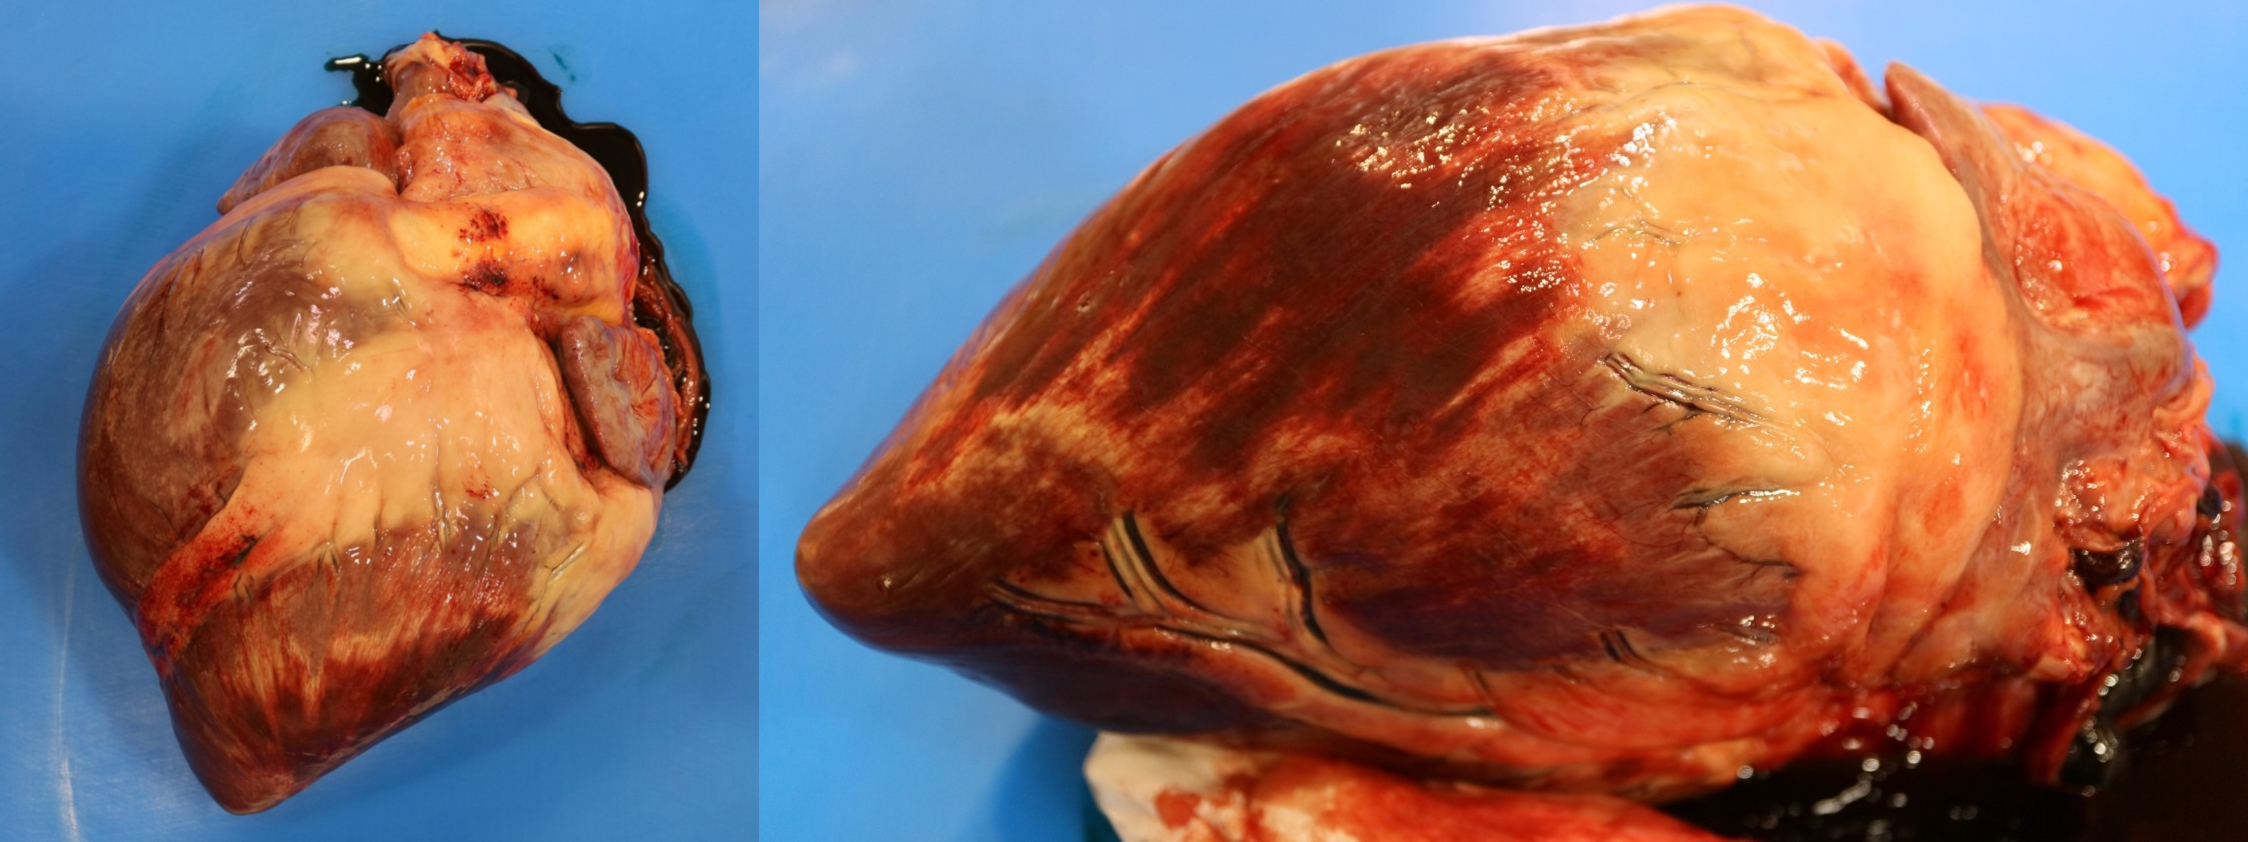
\includegraphics[width=0.6\linewidth]{images/heart-necrosis-comp} 

}

\caption{Necrosis of the myocardium. Pale white streaks bordered by hemorrhage are visible throughout the ventricle. Photo: C. Martin}\label{fig:heart-necrosis}
\end{figure}

The outcome of muscle damage and necrosis is dependent on its severity.
A structure known as the basal lamina plays an important role. The basal
lamina is a thin layer of extracellular matrix that keeps satellite
cells closely associated to the myofiber, and just importantly, keeps
fibroblasts out. If the basal lamina remains intact, and the damage only
affects a small portion of the myofiber, then muscle can regenerate.
These two criteria (intact basal lamina, focal area of damage) determine
whether or not a muscle will regenerate or undergo fibrosis.

Although myofiber nuclei themselves cannot divide, recall that each
myofiber is accompanied by \textbf{satellite cells} (a type of stem
cell), which can divide and differentiate into myofibers, \textbf{and
are critical components of muscle regeneration}. The steps in muscle
regeneration are fairly straightforward:

\begin{enumerate}
\def\labelenumi{\arabic{enumi}.}
\tightlist
\item
  Segmental injury or necrosis
\item
  Invasion of the sarcoplasm by circulating monocytes, which
  differentiate into macrophages.

  \begin{enumerate}
  \def\labelenumii{\roman{enumii})}
  \tightlist
  \item
    Macrophages phagocytose cellular debris, ``cleaning'' up the
    sarcoplasm.
  \end{enumerate}
\item
  Satellite cells enter the sarcoplasm and migrate towards the center of
  the of the myofiber.
\item
  Satellite cells divide and form a tube (``myotube'') which produces
  sarcoplasm.

  \begin{enumerate}
  \def\labelenumii{\roman{enumii})}
  \tightlist
  \item
    The myotube extends to the edges of the damaged myofiber.
  \item
    The myotube expands, though is still narrower than the unaffected
    myofiber.
  \item
    A row of nuclei appear in the center of the regenerating myofiber,
    and sarcomeres begin to form.
  \end{enumerate}
\end{enumerate}

Note that if the basal lamina has been destroyed, or if the damage
affects a large area, then regeneration does \emph{not} occur, and
instead the muscle repairs itself via fibrosis (scarring).

Segmental necrosis and regeneration occur following a variety of
insults, most commonly metabolic, nutritional (e.g.
\protect\hyperlink{selenium-and-vitamin-e-deficiency}{Selenium and
vitamin E deficiency}), or toxic (e.g.
\protect\hyperlink{ionophore-toxicity}{Ionophore toxicity})).
Determining the etiology of the damage can therefore be quite difficult.
It is helpful to observe the temporal pattern of the damage: are all
muscle fibers at the same stage of necrosis or regeneration, suggesting
a single, massive insult? Or is there a range of changes, with some
fibers showing early stages of necrosis, and others at the end of
regeneration, which suggests an on-going injury? These temporal changes
are known as \textbf{monophasic} (occuring at one point) or
\textbf{polyphasic} (an on-going proceess). These can be further
classified by the commonly used distribution modifiers: focal, locally
extensive, multifocal, or diffuse, to help narrrow down the etiology.
For example, a focal, monophasic injury is more likely to be traumatic
in origin than metabolic, while a multifocal, polyphasic injury could be
due to the on-going lack of a nutritional requirement, as seen in
\protect\hyperlink{selenium-and-vitamin-e-deficiency}{Selenium and
vitamin E deficiency}.

\section{Gross evaluation of muscle}\label{gross-evaluation-of-muscle}

Although important, the gross examination of muscles during a necropsy
can be underwhelming, and if muscular disease is suspected, samples of
muscle should \emph{always} be submitted for histopathology, regardless
of appearance. During a gross examination of a carcass, muscles should
be evaluated for changes in size, texture, and colour. Muscles can be
bigger (hypertrophied) or, more commonly, smaller (atrophied), or
normal. Difficulty in assessing the normal size of muscles for different
species and breeds can be aided by comparing with normal animals, or, if
unilateral disease is present, with the contralateral side.

Changes in the colour of muscle are common, are often artifactual, and
are dependent on blood perfusion, age, and species. Possible colour
changes, along with potential causes, are listed below.

\begin{itemize}
\tightlist
\item
  Pale muscles:

  \begin{itemize}
  \tightlist
  \item
    Normal in young animals
  \item
    Common in anemic animals
  \item
    Can be due to necrosis (ischemic)
  \item
    Denervation
  \item
    If streaking observed, usually due to necrosis and mineralization
    (e.g.~Figure \ref{fig:heart-necrosis}).
  \end{itemize}
\item
  Dark red:

  \begin{itemize}
  \tightlist
  \item
    Congestion or hemorrhage
  \item
    Hemorrhagic necrosis
  \item
    Inflammation
  \item
    Hypostatic congestion (i.e.~blood pooling due to gravity, a common
    artifact found during postmortem examinations)
  \end{itemize}
\item
  Green:

  \begin{itemize}
  \tightlist
  \item
    Putrefaction (rot)
  \item
    Eosinophilic inflammation (rare -- see
    \protect\hyperlink{sarcocystosis}{Sarcocystosis})
  \end{itemize}
\end{itemize}

The texture of diseased muscle can range from soft to hard
(mineralized). Soft muscle can be indicative of necrosis, or potentially
fat infiltration.

\section{Biopsy techniques}\label{biopsy-techniques}

As noted above, a biopsy of muscle should always accompany any suspected
muscular disease. Muscle is highly susceptible to artifact, but proper
preparation of the sample can help in ensuring a diagnostic sample.
Muscle retains the ability to contract after biopsy/death, and this
contraction can result in artifactual histological changes that mimic
true pathological changes. These changes, noted as \emph{contraction
band artifact}, can be prevented relatively easily: shortly after
removal, secure the muscle to a rigid surface prior to fixation. A
simple and manageable technique whether in the field or clinic is to
place a strip of muscle along a tongue depressor, and anchor it into
place using two needles, staples, or sutures, prior to placing the
sample in formalin. As a general rule, a muscle biopsy should not exceed
\textasciitilde{} 1 cm in diameter (with myofibers running lengthwise).

Note: if submitting a sample of muscle with sharps in the container,
make sure to notify the pathologist on the submission form.

\begin{figure}

{\centering \includegraphics[width=0.6\linewidth]{images/bx-technique} 

}

\caption{Appropriate technique for submitting muscle biopsies. A. Supplies that are readily available in most veterinary practices: a tongue depressor, broken to the appropriate size, and two small gauge needles. B. The diameter of a muscle biopsy should not exceed approximately 1 cm. C. Affix the biopsy to the tongue depressor using the two needles, staples, or sutures. Only a small amount of force is required to secure the muscle to the wood.}\label{fig:bx-technique}
\end{figure}

\chapter{Congenital and inherited
myopathies}\label{congenital-and-inherited-myopathies}

This is a large group of conditions, and several are commonly seen in
veterinary species. Congenital conditions tend to be evident at, or soon
after, birth, but are \emph{not} necessarily inherited. Inherited
conditions indicate an underlying genetic etiology, but do not
necessarily mean that the parents are also affected.

\section{Primary central nervous system
conditions}\label{primary-central-nervous-system-conditions}

Muscles of the developing embryo require normal innervation in order to
develop properly. Lack of normal innervation can lead to atrophy or
replacement with fibrous connective tissue. Recall that motor neurons
release trophic factors at the motor end plate that are critical to the
health of skeletal muscle . Conditions that primarily affect the motor
neurons, therefore, can have significant effects on skeletal muscle.

\subsection{Arthrogryposis}\label{arthrogryposis}

Arthrogryposis refers to the abnormal angulature of the limbs
(\emph{arthro}: joint; \emph{gryposis}: abnormal curvature). As you
might expect, this condition is evident immediately at birth, and can
affect one or more limbs in a multitude of different ways: they may be
rotated, curved backwards or forwards, or abducted. The curve of the
vertebral column may be affected as well: scoliosis (\emph{lateral}
deviation), kyphosis (\emph{dorsal} deviation), or torticollis (twisted
neck) are not uncommon. Muscle mass is reduced.

The causes of arthrogryposis are varied but are often unclear. There is
a distinct association with \textbf{dysraphism} -- the arrest or delayed
closure of the neural tube (e.g.~spina bifida) -- and arthrogryposis.
Other causes include toxins (e.g.~wild lupine) and a variety of viruses,
including the Orthobunyaviruses (Schmallenberg, Cache Valley, and
Akabane viruses), bluetongue virus, and border disease virus.

\section{Muscular defects}\label{muscular-defects}

\subsection{Splayleg}\label{splayleg}

Splayleg is an odd condition that occurrs only in neonatal piglets
(Figure \ref{fig:splayleg}). Piglets are born unable to adduct their
limbs (particularly the hindlimbs) and are often found in a
characteristic ``splayed'' position. The cause is unknown, but is
thought to be associated with immature skeletal muscle present at the
time of birth. Importantly, the condition is \emph{transient}: all
animals make a full recovery within 1, or at most 2, weeks. While
affected, however, the animals are at risk of accidental injury and may
become malnourished due to difficulty in nursing.

\begin{figure}

{\centering 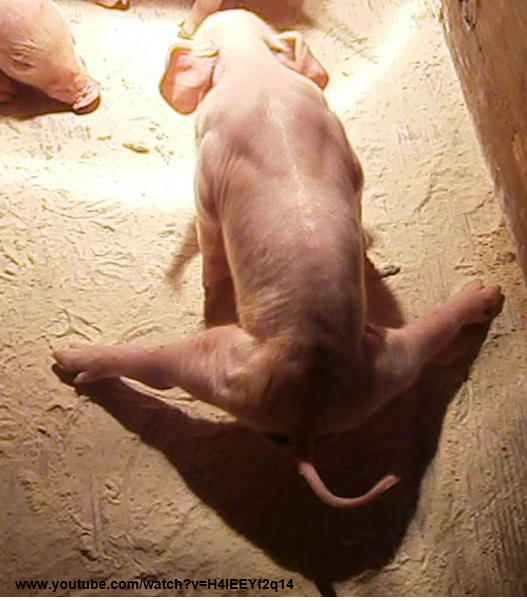
\includegraphics[width=0.6\linewidth]{images/splayleg} 

}

\caption{Piglet affected by splayleg}\label{fig:splayleg}
\end{figure}

\subsection{Muscular hyperplasia}\label{muscular-hyperplasia}

Recall that normal muscle \emph{cannot} undergo hyperplasia: increase in
muscle size is usually a function of hypertrophy. However, myofiber
hyperplasia is the hallmark of a defective protein known as myostatin.
Myostatin is a protein produced and released by myofibers and normally
\emph{inhibits} muscle growth. Genetic defects in the myostatin gene,
resulting in dysfunctional myostatin, result in hyperplasia of skeletal
muscle, known as ``double muscling''. As this is \emph{hyperplasia},
muscles have increased numbers of structurally normal myofibers. This
trait has been selected for in several beef breeds, including Belgian
Blue (Figure \ref{fig:belgian-blue}) and White. The condition is also
seen in Whippet dogs (``bully'' Whippets). Muscular hyperplasia is most
pronounced in the thighs, rumps, loins, and shoulders.

\begin{figure}

{\centering 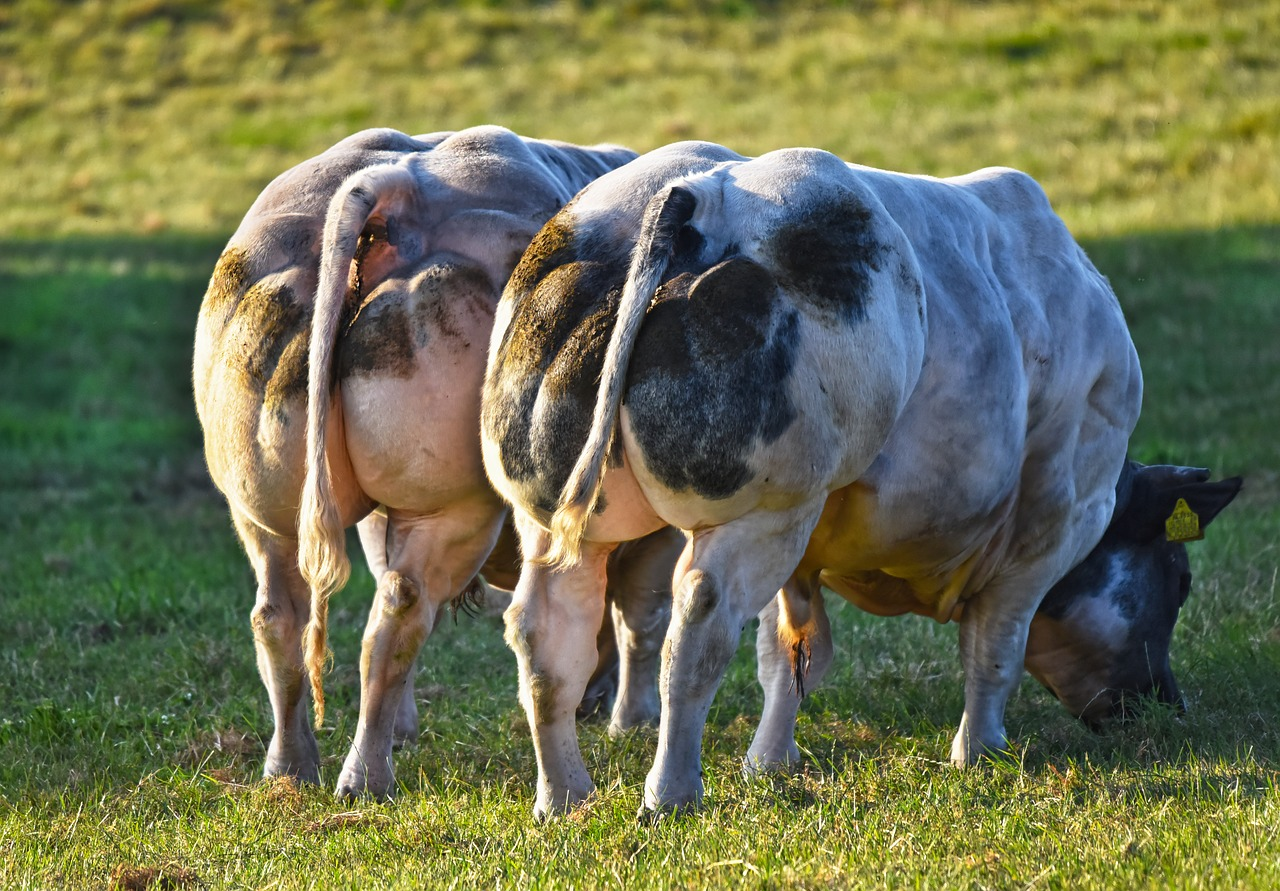
\includegraphics[width=0.6\linewidth]{images/belgian-blue} 

}

\caption{Two Belgian Blue cattle showing marked muscular hyperplasia of the rump.}\label{fig:belgian-blue}
\end{figure}

\subsection{Steatosis}\label{steatosis}

Steatosis of muscles refers simply to the replacement of myofibers by
adipocytes, usually following damage or denervation. It is generally
considered an incidental finding at necropsy, but does sometimes raises
concern at meat inspection.

\subsection{Congenital diaphragmatic
clefts}\label{congenital-diaphragmatic-clefts}

Abnormal closure of the developmentally complex diaphragm can result in
congenital diaphragmatic hernias. They have been reported most
frequently in the dog and rabbit.

\section{Muscular dystrophies}\label{muscular-dystrophies}

Muscular dystrophies (as defined in the human literature) are
\textbf{inherited} conditions characterized by \textbf{progressive
myopathy with necrosis and regeneration of myofibers}. Be aware that the
term dystrophy is commonly misused in veterinary medicine, and only a
few true dystrophies have been described, notably in the dog, cat, and
sheep. These conditions typically manifest in young animals and
progressively worsen as the animal ages. The canine and feline X-linked
dystrophies are analagous to Duchenne and Becker muscular dystrophies of
humans. Both are related to a mutation in the gene encoding dystrophin,
a cytoskeletal protein. The pathogenesis of muscle damage in both
conditions is poorly understood.

\subsection{X-linked dystrophies of dogs and
cats}\label{x-linked-dystrophies-of-dogs-and-cats}

The X-linked dystrophies of dogs and cats share several similarities and
a few key diferences, summarized below in Table
\ref{tab:dystrophy-table}. Both conditions affect the dystrophin
protein, whose exact function is still somewhat uncertain. Because
affected gene is found on the X chromosome, \emph{males} are
overrepresented. Note that the level of detail presented here is beyond
what you would be expected to know on an exam.

\begin{table}[t]

\caption{\label{tab:dystrophy-table}Comparison of canine and feline X-linked dystrophy}
\centering
\begin{tabular}{l>{\raggedright\arraybackslash}p{15em}>{\raggedright\arraybackslash}p{15em}}
\toprule
  & Canine & Feline\\
\midrule
Breed predisposition & Golden retrievers, but also described in many others & Mixed breeds\\
Sex predisposition & Male & Male\\
Effect on muscle & Atrophy & Hypertrophy\\
Clinical signs & Progressive muscular weakness, abnormal gait, regurgitation & Stiff gait with 'bunny hopping', difficulty jumping, regurgitation. May be subtle.\\
Serum biochemistry & Increased CK, AST & Increased CK, AST\\
\addlinespace
Gross findings & Severe cases: marked degeneration with pale white streaks of the diaphragm and strap muscles & Marked thickening of the esophagus and contraction of the diaphragm. Muscle is often pale, and there may be pale streaks in the myocardium.\\
Histologic findings & Myofiber atrophy, necrosis, regeneration & Marked variation in myofiber size including marked hypertrophy. Necrosis and regeneration are present.\\
Endomysial fibrosis & May be marked & Mild\\
Cardiac changes & Subepicardial necrosis, mineralization, and fibrosis leading to CHF & Necrosis and mineralization with fibrosis that typically does NOT result in clinical symptoms.\\
\bottomrule
\end{tabular}
\end{table}

\subsection{Ovine muscular dystrophy}\label{ovine-muscular-dystrophy}

Unlike the X-linked dystrophies of dogs and cats, ovine muscular
dystrophy is an \textbf{autosomal recessive} condition that affects
males and females equally. The condition is still common in Merino sheep
in Australia, with 1-2\% of animals showing signs of the disease.
Clinical signs include a lack of normal growth, abnormal gait, and/or
stiffness. Most animals will show clinical signs by 1 year of age, and
be severely affected by 2-3 years old. If left at unattended at pasture,
severely affected animals are so weak that they die of starvation.

Gross changes include emaciation and replacement of muscles with adipose
tissue. Histologically there are characteristic amphophilic sarcoplasmic
masses and large, vesicular nuclei.

\section{Metabolic myopathies}\label{metabolic-myopathies}

Metabolic abnormalities are typically inherited, and abnormal metabolism
can lead to abnormal function of muscle. There are a large number of
metabolic diseases. Some affect enzymes present in multiple organs,
including skeletal muscle, while others affect enzymes or isoenzymes
solely in muscle. The defects are often related to issues in
\textbf{processing or storing of glycogen}. Many of these conditions are
rare and relatively breed specific (for example, include glycogen
storage disease type II in dogs and glycogen storage disease type IV in
Norwegian Forest cats and horses). These uncommon conditions will not be
discussed further here, but more information can be found in the
reference textbooks. Instead, we will focus on a common metabolic
myopathy of horses known as polysaccharide storage myopathy.

\hypertarget{equine-polysaccharide-storage-myopathy-pssm}{\subsection{Equine
polysaccharide storage myopathy
(PSSM)}\label{equine-polysaccharide-storage-myopathy-pssm}}

Equine polysaccharide storage myopathy (PSSM) is seen with some
frequency in horses. Although Quarter horses, Warmbloods, and Draft
horses are overrepresented, PSSM has been reported in almost all breeds.
As it's name suggest, PSSM is a glycogen storage myopathy. It is an
inherited, autosomal dominant disease with variable clinical expression.
One form of the disease has been linked to a mutation in the glycogen
synthase I gene, for which a genetic test is now available, but not all
cases of PSSM are caused by this mutation.

The pathogenesis of PSSM is still poorly defined, but is characterized
by the abnormal accumulation of glycogen in myofibers, predominantly of
the type 2 variety. A specific abnormality explaining abnormal
utilization of intracytoplasmic glycogen has yet to be found, but a
metabolic defect is still suspected.

Horses with PSSM present with a variety of clinical signs. Unexplained
pelvic limb lameness is the most common finding. Horses may also have a
stiff gait, sore back, muscle cramping, and/or muscle weakness. Some
horses may present with recurrent episodes of
\protect\hyperlink{equine-exertional-rhabdomyolysis}{exertional
rhabdomyolysis}. Some horses with the condition may be subclinically
affected. Horses with PSSM are at increased risk of suffering from
\protect\hyperlink{postanesthetic-myopathy-of-horses}{post-anesthetic
myopathy}.

Gross findings may range from normal musculature to muscles with pale,
white, necrotic streaks. When present, lesions tend to be most notable
in muscles composed predominanlty of type 2 fibers: the
\textbf{semimembranosus, semitendinosus}, and gluteals, for example.
Biopsies of the semimebranosus and semitendinosus muscles are good
choices for the diagnosis of PSSM. In cases of sudden death, the
diaphragm should be carefully examined, as severe myonecrosis may have
occurred. Along with microscopic evidence of polyphasic, multifocal
necrosis, myofibers contain notable intrasarcoplasmic, PAS-positive
inclusions (Figure \ref{fig:PSSM}).

\begin{figure}
\centering
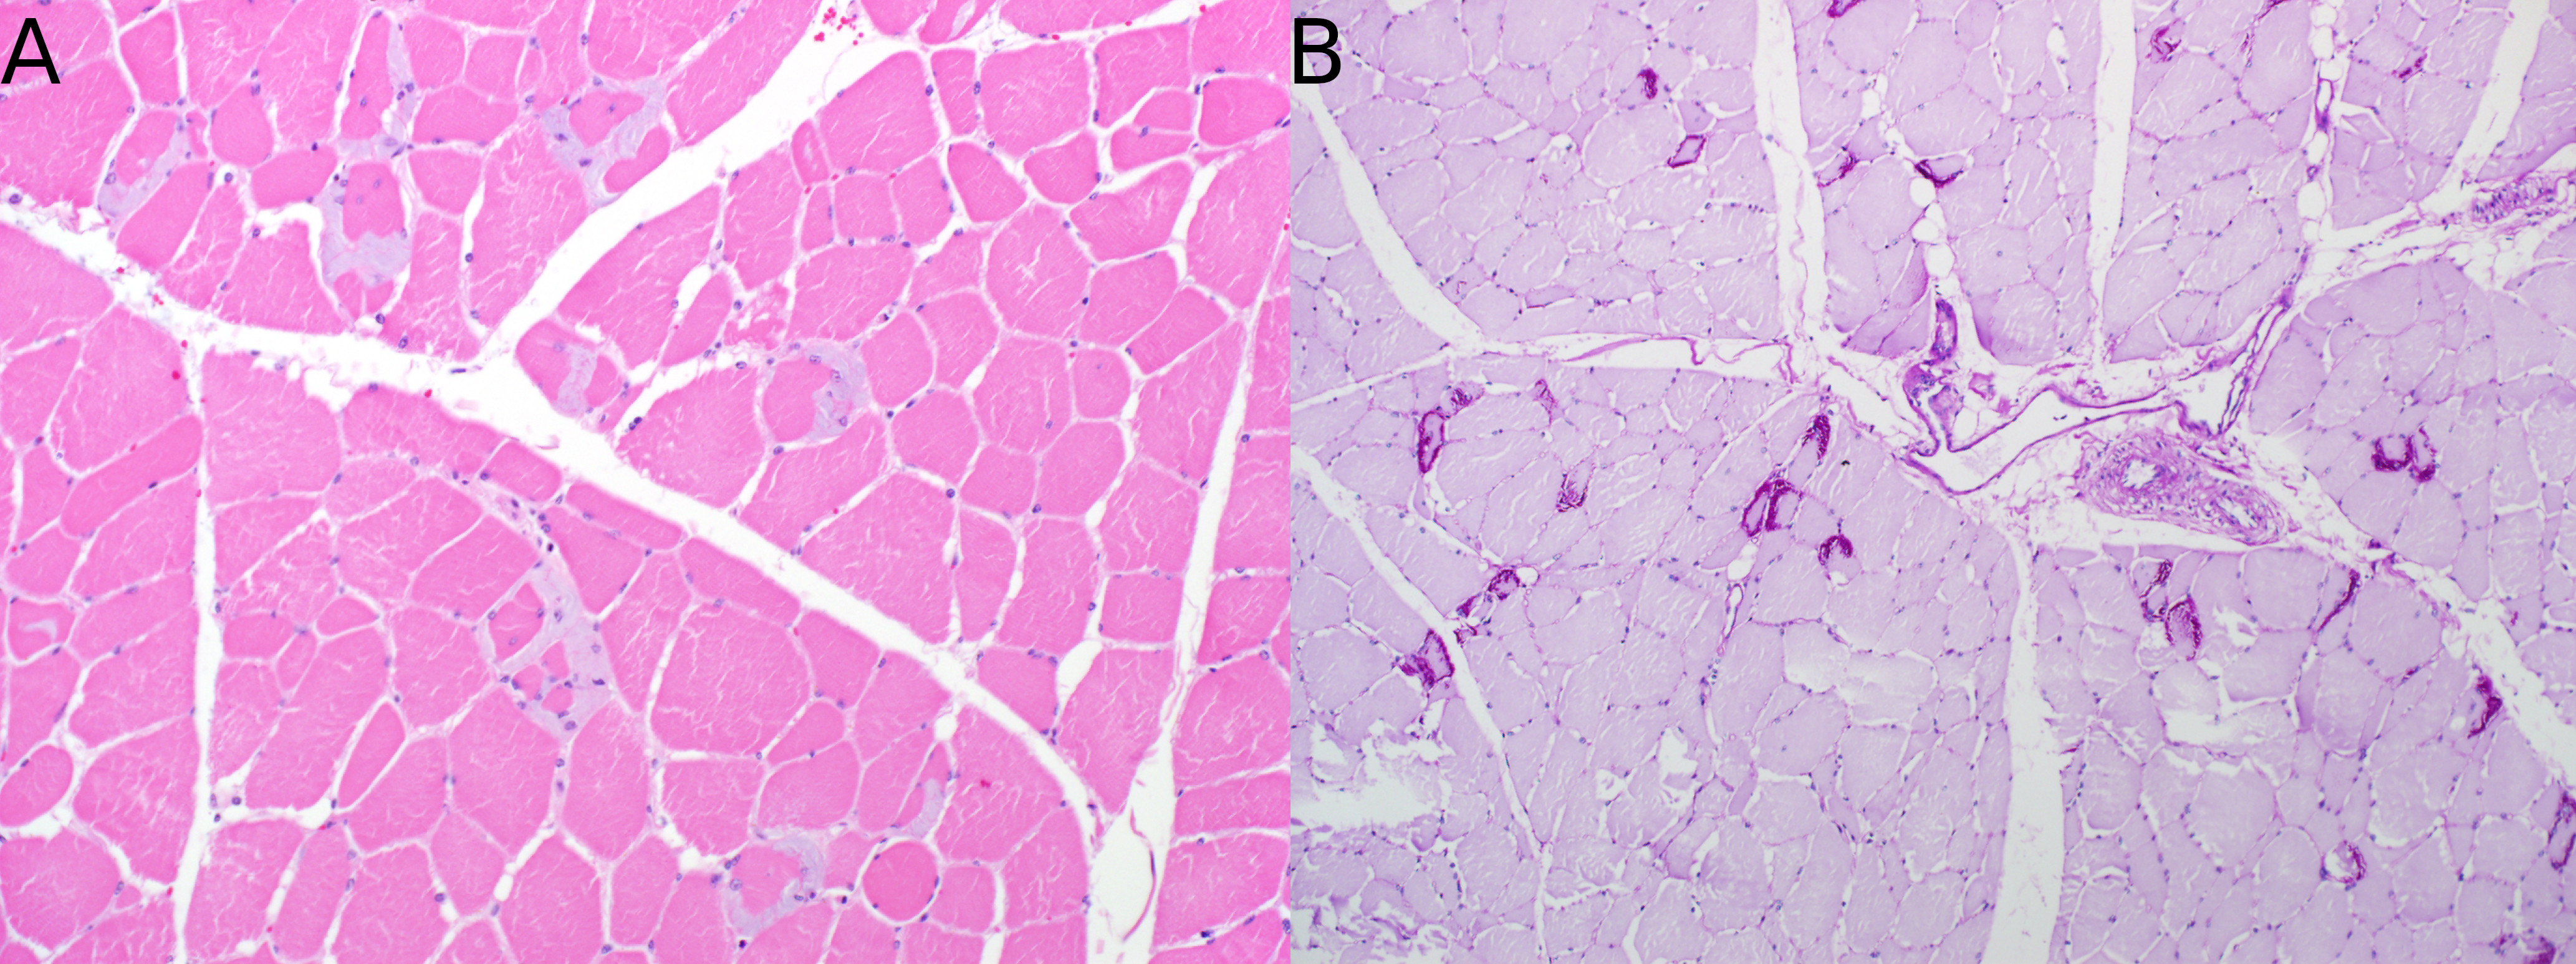
\includegraphics{images/PSSM.jpg}
\caption{\label{fig:PSSM}Photomicrograph of muscle from a horse with PSSM.
A) Multiple myofibers show distinct amphophilic material, particularly
along the periphery of the myofiber. H\&E B) The material stains
positive with PAS (bright magenta). PAS.}
\end{figure}

\section{Malignant hyperthermia}\label{malignant-hyperthermia}

Though clasically thought of as a disease of pigs, malignant
hyperthermia is better thought of as a syndrome that predominantly
occurs in swine, but which also affects dogs and horses. The underlying
issue is a defect in the \emph{RYR1} gene, which encodes the ryanodine
receptor, a calcium channel present within the sarcoplasmic reticulum.
Defective ryanodine receptors are responsible for the release of
Ca\textsuperscript{2+} during contraction. Defective ryanodine receptors
stay open for longer, leading excess Ca\textsuperscript{2+} release,
prolonged contraction, hypercontraction, and hyperthermia.

\subsection{Porcine stress syndrome}\label{porcine-stress-syndrome}

Malignant hyperthermia is best characterized in pigs, and is also known
as porcine stress syndrome (PSS). It is the cause of pale, soft, and
exudative pork that is sometimes encountered at slaughter. A single
nucleotide polymorphism in the \emph{RYR1} gene of pigs is the cause. It
is estimated that between 2-30 \% of pure-bred pigs are susceptible to
PSS.

Pigs may be unaffected or subclinical. Stressful events (such as
fighting or transport), or halothane anesthesia, however, can trigger
severe episodes in which pigs display intense limb and torso rigidity,
hyperthermia, tachycardia, dyspnea, metabolic acidosis, and rapid death.
Gross lesions are related to the increased body temperature: classically
pale, soft, exudative muscle (meat). Lesions attritutable to heart
failure, including pulmonary edema, hydrothorax, and hepatic congestion,
may occur if the animal survives the acute episode. Histologically,
multifocal, monophasic necrosis is present, and edema separates
myofibers in animals that have suffered from hyperthermia.

\hypertarget{congenital-myasthenia-gravis}{\section{Congenital
myasthenia gravis}\label{congenital-myasthenia-gravis}}

Myasthenia gravis is a neuromuscular disorder characterized by decreased
availability of acetylcholine (Ach) receptors (Ach-R) on the myofiber
membrane. Lack of the receptor leads to decreased Ach binding, fewer
depolarizations, and weaker muscle contractions. In congenital
myasthenia gravis, decreased Ach-R availability is due to an inherent
defect in the receptor. In
\protect\hyperlink{acquired-myasthenia-gravis}{acquired myasthenia
gravis}, circulating autoantibodies bind to and block the binding of Ach
to their receptor. \textbf{The acquired form is much more common than
it's congenital counterpart.}

In dogs, congenital myasthenia gravis is autosomal recessive. Puppies
develop exercise-induced collapse by 5-16 weeks of age, depending on
breed. Regurgitation secondary to megaesophagus is a common clinical
finding. Antibodies against Ach-R cannot be demonstrated.

The disorder is even less common in cats, which may seem normal at
birth, but by approximately 4-5 months of age show signs of episodic
weakness. Megaesophagus is \emph{not} a feature. The condition remains
poorly characterized.

\section{Myotonic and spastic
syndromes}\label{myotonic-and-spastic-syndromes}

\textbf{Myotonia} is the temporary inability of muscles to relax. It can
be acquired or inherited; in veterinary species, the inherited form is
most common. Three are a variety of myotonias in dogs, cats, and goats
that will not be covered here; more information can be found in the
reference textbooks.

\hypertarget{hyperkalemic-periodic-paralysis-hypp}{\subsection{Hyperkalemic
periodic paralysis (HYPP)}\label{hyperkalemic-periodic-paralysis-hypp}}

Only horses descended from the Quarter Horse stallion ``Impressive'' are
at risk for HYPP. Affected animals have very well defined musculature, a
desireable trait, which has led to the propogation of the condition in
the quarter horse breed.

The pathogenesis of the condition is poorly understood. The underlying
cause is a defect in Na\textsuperscript{+} channels causing excess
influx of Na\textsuperscript{+} and efflux of K\textsuperscript{+} from
myofibers. This alters the membrane potential of myofibers and leads to
increased and prolonged action potentials, and excess contractile
activity.

The condition presents differently depending on whether the animal is a
heterozygote or homozygote. Homozygote foals characteristically suffer
from laryngospasm, which can generate a distinctive inspiratory noise.
They may develop dysphagia and become emaciated during their first 2
years. The larynx may collapse with exercise. Homozygotes typically do
not survive beyond 2 years of age.

Heterozygotes are less severely affected, and often appear normal but
suffer from transient attacks of muscle fasiculations and spams
(myotonia), inspiratory stridor, protrusion of the third eyelid, and
sometimes followed by acute paralytic collapse. Sudden death may occur
in the most severe cases.

There are no gross or histologic lesions; diagnosis is based on
ancestry, clinical history, signs, and DNA testing. Despite the name,
hyperkalemia is not a consistent finding.

\chapter{Circulatory disturbances}\label{circulatory-disturbances}

Due to the high demand for oxygen and nutrient, skeletal muscle is a
relatively well vascularized tissue (as you will find out when you cut a
muscle belly during surgery!). This makes it somewhat resistant to
vascular injury, as there is substantial collateral circulation: each
myofiber is supplied by 3-12 capillaries. Thus, for the most part,
ischemic damage to muscle is due to pressure over \emph{large} surfaces
of the body. Thromboembolic occlusion of a large vessel, most commonly
seen at the aortoiliac junction in cats (and horses), can also lead to
ischemic necrosis of large areas of muscle.

\section{Compartment syndrome}\label{compartment-syndrome}

Compartment syndrome occurs most commonly in chickens (and humans). As
discussed in the \protect\hyperlink{the-anatomy-of-muscle}{review of
muscule anatomy}, muscles are covered by various layers of connective
tissue. Some muscles -- the \textbf{supracoracoid muscles in chickens},
for example -- are surrounded by inelastic tissues. In the case of the
supracoracoid, the muscle is contained by the breastbone on one side,
and a relatively rigid outer sheath on the other, forming an inelastic
or fixed ``compartment''. When a chicken participates in short, vigorous
exercise (wing flapping), there is a significant increase intramuscular
vascular pressure that collapses veins and decreases venous outflow. On
top of this, muscle contraction can increase the diameter of myofibers
by 20\%, and in a restricted compartment, this contributes to further
venous collapse. Increased muscular activity also increases arterial
blood flow. The net result is increased arterial flow with decreased
venous outflow leading to ischemic necrosis, all caused by a muscle held
captive by rigid surrounding tissues. Damage to vessels subsequent to
the necrosis can lead to interstitial edema, further increasing tissue
pressure, and exacerbating the condition. Treatment (generally for
humans) can involve a fasciotomy to relieve the pressure.

\section{Downer syndrome}\label{downer-syndrome}

Downer syndrome refers to ischemic myopathy caused by long periods of
recumbency, leading to undue pressure on the dependent muscles. Size and
weight of the animal are important factors: larger, well muscled animals
are more prone to this syndrome than are thin animals. Cows are most
frequently affected, while cats seem to be exempt.

The pathogenesis is more complicated than initially meets the eye. The
increased pressure on muscles caused by prolonged recumbency initially
collapses veins, causing congestion and ischemia. Eventually arteries
are affected as well, further contributing to the ischemic damage. If
and when the animal changes positions and relieves the pressure,
arteries are the first to recover, and the increased arterial pressure
in the face of decreased venous outflow leads to edema, which itself can
cause increased pressure and decreased venous outflow, further
compounding the problem. Reperfusion injury also likely contributes to
muscle damage.

\hypertarget{postanesthetic-myopathy-of-horses}{\section{Postanesthetic
myopathy of horses}\label{postanesthetic-myopathy-of-horses}}

Horses that undergo prolonged anesthesia are prone to ischemic myopathy,
especially if inadequate padding is used. Pressure on the muscle
capillaries, caused by the weight of the horse, exceeds the pressure of
perfusion, resulting in ischemia. The muscles affected depend on the
position of the horse. Predisposing factors include intraoperative
hypotension and the presence of comorbities, especially
\protect\hyperlink{equine-polysaccharide-storage-myopathy-pssm}{PSSM}
and \protect\hyperlink{hyperkalemic-periodic-paralysis-hypp}{HYPP}.

\chapter{Physical injuries}\label{physical-injuries}

Traumatic injuries to muscle include lacerations, penetrating wounds,
tears, and strains are common in domestic species. Their pathogenesis is
straightforward, and the outcome depends on the severity of the trauma.

A muscle rupture can occur following violent exercise or trauma. The
muscle forms a bulge at the end opposite of the rupture. The most
commonly ruptured muscle is the diaphragm, particularly after traumatic
injury (e.g.~hit by car). Healing is usually by fibrosis, as the damage
is usually too extensive for regeneration to occur.

A muscle strain is the overextension of muscles resulting in myofiber
disruption, particularly at the junction with tendons. Severity varies,
and healing is by fibrosis.

The physical consequences of penetrating wounds are self-explanatory,
but you should also be aware that secondary complications, such as
\protect\hyperlink{suppurative-myositis}{bacterial infection} or
\protect\hyperlink{tetanus}{tetanus}, may result.

\chapter{Nutritional myopathies}\label{nutritional-myopathies}

\hypertarget{selenium-and-vitamin-e-deficiency}{\section{Selenium and
vitamin E deficiency}\label{selenium-and-vitamin-e-deficiency}}

Deficiency in selenium, and to a lesser extend, vitanim E, is a
\textbf{very important} disease of young cattle, sheep, swine, and
horses. Neonatal animals are particularly susceptible, as they rely on
stores accumulated \emph{in utero}, which may be sub-optimal. The
disease is rarely seen in carnivores. This disease is also colloquially
known as \textbf{white muscle disease}. Selenium and vitamin E levels in
animals are directly related to dietary intake, it is thus important
that animals are fed well balanced rations. Complicating matters,
vitamin E degrades over time, and feed that was originally properly
formulated may wind up being low in vitamin E if stored for prolonged
periods.

\textbf{Selenium and vitamin E are components of antioxidants} that play
important roles in the control of free radicals and oxidative damage.
Recall that a free radical is a molecule with an unpaired electron, and
as such are highly reactive and have enormous potential to damage cell
and mitochondrial membranes (lipid peroxidation). Antioxidants are
protective against free radicals: vitamin E directly scavenges free
radicals, while selenium is a component of an enzyme, glutathione
peroxidase, that reduces free radicals.

When levels of selenium and/or vitamin E are low, free radical damage
accumulates, particularly in skeletal and cardiac muscle. The high
oxygen requirement and contractile activity of these two tissues renders
them particularly susceptible to oxidative damage. Free radical damage
to cell and organelle membranes contributes to a loss of ionic gradient
and increased sarcoplasmic Ca\textsuperscript{2+} concentrations,
leading to hypercontraction, myofiber necrosis, and potentially
mineralization.

Grossly, the necrotic muscle appears \textbf{white}, though, if you
recall, this is a \emph{non-specific} finding, and could be the result
of a number of etiologies. When performing a necropsy, pay close
attention to muscles that tend to be the most active: the heart
(particularly the left ventricle of calves, right ventricle of sheep,
the tongue, diaphragm, and intercostal muscles). Histologically, there
is \emph{multifocal, polyphasic necrosis with regeneration}. The damage
tends not to affect the basal lamina or satellite cells, so myofibers
are able to regenerate and recover, depending on the severity of the
damage. Although regeneration is possible, it is not infrequent for
animals to die or be euthanized due to this condition.

\chapter{Toxic myopathies}\label{toxic-myopathies}

Skeletal muscle is a highly vascular and metabolically active tissue and
is therefore somewhat susceptible to a variety of toxins. The most
commonly encountered toxins in veterinary species are ionophore
antibiotics and plant associated toxins. Livestock and horses are most
frequently affected.

\hypertarget{ionophore-toxicity}{\section{Ionophore
toxicity}\label{ionophore-toxicity}}

Ionophore antibiotics are commonly found in the feed of livestock and
are used as growth promoters. Horses are particularly susceptible to
ionophore toxicity, requiring only low concentrations of the drug to
cause severe damage, and may be exposed either through errors at feed
mills or by consuming feed formulated for other species.
\textbf{Monensin} is the most frequently implicated ionophore.
Ionophores affect membrane permeability to electrolytes, and results in
calcium overload and subsequent death of skeletal and cardiac muscle.
Affected horses may show sings of colic, lethargy, stiffness, and/or
weakness. Lesions are often seen within 48 hours. The heart is often
most severely affected, showing pale, white to tan, often streaked areas
of necrosis (Figure \ref{fig:heart-necrosis2}); other muscles may show
similar changes, though to a lesser degree. Horses usually only require
one dose to become severely affected, and therefore show acute,
multifocal, monophasic muscle injury.

\begin{figure}

{\centering 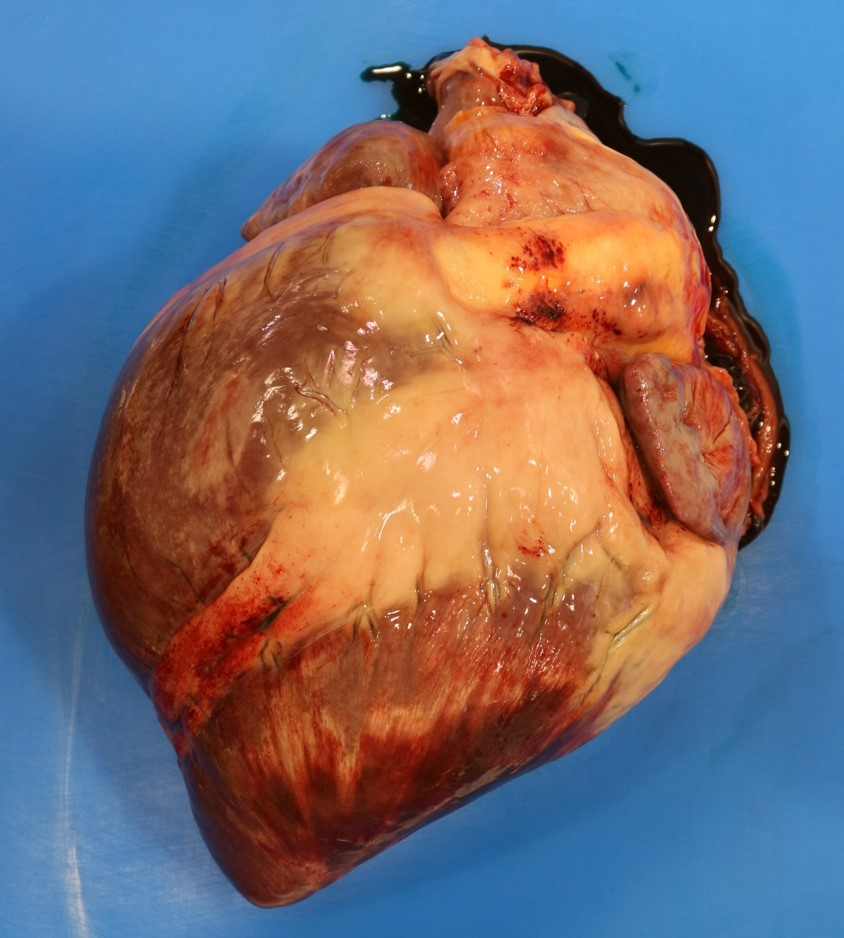
\includegraphics[width=0.3\linewidth]{images/heart-necrosis-2} 

}

\caption{Equine heart demonstrating marked myocardial necrosis, manifesting as pale white streaks across the ventricle. Photo: C. Martin}\label{fig:heart-necrosis2}
\end{figure}

\section{Plant toxicities}\label{plant-toxicities}

Gossypol from cottonseeds (\emph{Gossypium} spp.), senna or coffee senna
plant (\emph{Senna occidentalis}, formerly \emph{Cassia occidentalis} or
\emph{C. obtusifolia}), or coyotillo (\emph{Karawinskia humboldtiana})
are the most common sources of plant toxin-induced myopathy (Figure
\ref{fig:plants}). The latter two produce a rapidly progressing disease
characterized by a swaying, stumbling gait followed by recumbency,
myoglobinuria, and elevated CK. Mortality is high. Gross lesions include
ill-defined pallor of many muscles, that under light microscopy
demonstrate multifocal, monophasic myonecrosis. Cattle, horses and pigs
are particularly affected.

Gossypol toxicity occurs mostly in pigs. Cottonseed, the source of
gossypol, is added to swine feed as a protein supplement, and toxicity
occurs when excess cottonseed (\textgreater{} 10 \% of feed) is
consumed. Lesions take weeks to 1 month to appear, and include skeletal
and cardiac myonecrosis.

\subsection{Seasonal pasture myopathy of
horses}\label{seasonal-pasture-myopathy-of-horses}

Ingestion of box elder and/or sycamore maple tree seeds containing
hypoglycin A causes seasonal pasture myopathy of horses. This disease is
characterized by rhabdomyolysis and myoglobinuria, typically occurs in
the fall, and can be fatal. Gross findings are non-specific, typically
consisting of pale, necrotic muscles affecting multiple different
muscles.

\begin{figure}

{\centering 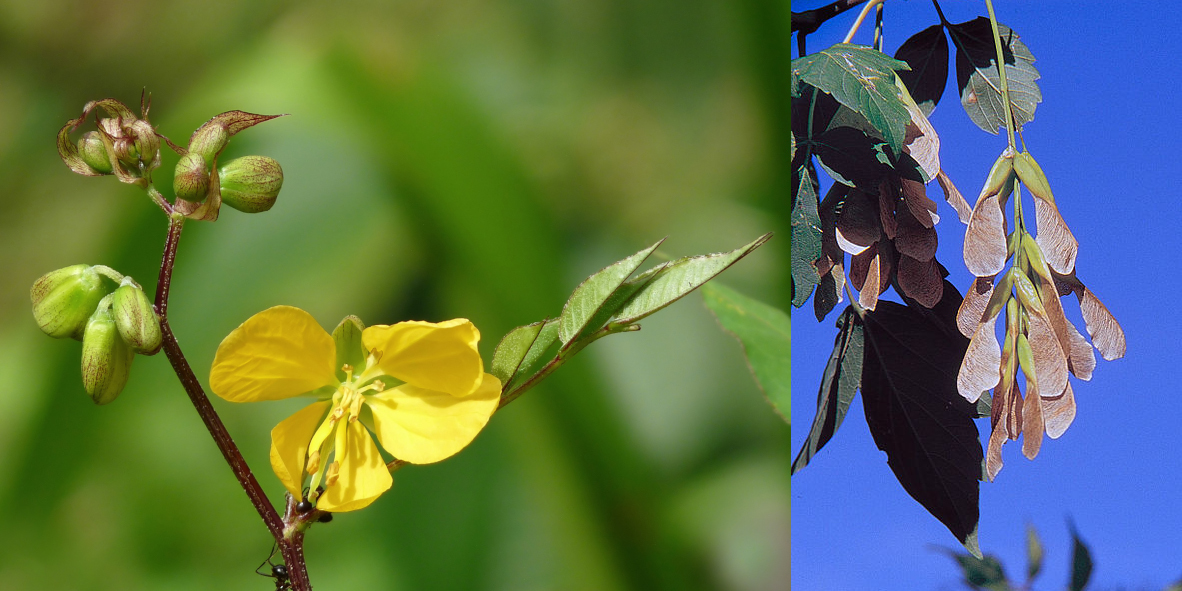
\includegraphics[width=0.6\linewidth]{images/plants} 

}

\caption{Left: A coffee senna plant. Photo by Jee and Rani Nature Photography (License: CC BY-SA 4.0, https://commons.wikimedia.org/w/index.php?curid=9452256). Right: Box elder (Manitoba) maple seeds.}\label{fig:plants}
\end{figure}

\chapter{Degenerative/necrotizing
myopathies}\label{degenerativenecrotizing-myopathies}

Although degeneration and necrosis are a feature of a number of
different myopathies, this section describes myopathies that \emph{do
not have a congenital, nutritional, toxic, or infectious} etiology.

\section{Exertional myopathies}\label{exertional-myopathies}

An exertional myopathy is defined as myofiber damage occuring as the
direct result of exercise.

\hypertarget{equine-exertional-rhabdomyolysis}{\subsection{Equine
exertional rhabdomyolysis}\label{equine-exertional-rhabdomyolysis}}

\emph{Synonyms: blackwater, Monday morning disease, set fast, paralytic
myoglobinuria, azoturia}

Exertional rhabdomyolosis is a significant disease of horses. It is
often worse in heavy, draft breeds as compared to light breeds, and
female horses are predisposed. The pathogenesis of the condition is not
completely known. The current accepted theory is that muscle damage is
most often due to underlying metabolic abnormalities, possibly a
post-exercise hypokalemia, and not management factors. Interestingly,
although diet is not considered to be the underlying cause of exertional
rhabdomyolysis, virtually all horses suffering from the condition
respond favourably to a diet high in fat and fiber and low in starches.

Exertional rhabdomyolysis presents as a sudden onset of weakness, pain,
and discomfort, sometimes with tremors or sweating, during or after
periods of exercise. The exercise does not have to be overly strenuous
or exhaustive. Severe cases may progress to recumbency. Type 2
glycolytic myofibers are most severely affected. Cardiac muscle is
spared, and mineralization is not a feature. Grossly, affected muscles
(particularly the gluteal, femoral, and lumbar muscles) may be swollen
and dark red, with streaks of pale pallor present in severe cases.
Histologically there is necrosis of type 2 fibers. Fibrosis and atrophy
will be present in chronic cases. Myoglobinuria is a common feature, and
can lead to myglobinuric nephrosis.

There is evidence that horses with
\protect\hyperlink{equine-polysaccharide-storage-myopathy-pssm}{PSSM}
are predisposed, but the exact mechanism is unclear.

\subsection{Canine exertional
rhabdyomyolysis}\label{canine-exertional-rhabdyomyolysis}

As one might expect, this syndrome appears most frequently in racing
dogs, namely Greyhounds and sled dogs. It is not particularly well
understood, but thought that separate mechanisms cause the syndrome in
sprinting versus endurance racing. In Greyhounds, clinical signs and
symptoms are similar to those noted for horses, while in sled dogs may
present with sudden death.

\subsection{Capture myopathy}\label{capture-myopathy}

This is a syndrome seen both in free and captive wildlife. The stress of
capture, which is usually preceeded by a chase and/or struggle in these
animals, results in a combined massive release of catecholamines and
overexertion that is frequently fatal. Muscles may be pale and edematous
or may show pale streaks with hemorrhage. Degeneration and necrosis is
frequently observed histologically. This condition is extremely
important in zoological collections, and as such great care is often
taken when tranquilizing or restraining animals for examination.

\chapter{Myopathies associated with serum electrolyte
imbalance}\label{myopathies-associated-with-serum-electrolyte-imbalance}

\section{Feline hypokalemia}\label{feline-hypokalemia}

Hypokalemia in cats can lead to a distinct clinical syndrome called
feline hypokalemic polymyopathy. It is characterized by ventroflexion of
the neck, a stiff, stilted gait, muscle pain, reluctance to walk, and
weakness. Low potassium can be the result of decreased dietary intake,
chronic renal disease, or in cats fed acidifying diets to control
urolithiasis. The pathogenesis of muscle injury in hypokalemia is
attributed to a decrease in resting membrane potential of myofibers,
atlerted glycogen metabolism, and ischemia from hypokalemia-induced
vasocontriction. Frustratingly, lesions can be mild or absent in
clinical cases. Histologic lesions are most likely to be found in
\textbf{respiratory muscles -- the intercostals and the diaphram } --
and these are recommended for sampling at autopsy if the disease is
suspected.

\section{Bovine hypokalemia}\label{bovine-hypokalemia}

Rather specifically, muscle weakness has been observed in cattle being
treated with isoflupredone for ketosis. The drug can cause severe
hypokalemia. These animals are weak and recumbent. Acute necrosis occurs
in both weight- and non-weight bearing muscles.

\chapter{Immune-mediate myopathies}\label{immune-mediate-myopathies}

Generally speaking, immune-mediated disease is the result of abnormal
immune response against self-peptides or antigens.

A difficulty when evaluating immune-mediate disease is determining
whether the immune response is the primary \emph{cause} of muscle
damage, or whether the leukocytes are simply \emph{responding} to the
damage. In the case of immune-mediate myopathies, the invasion of intact
myofibers by mononuclear leukocytes is characteristic.

\section{Masticatory myositis}\label{masticatory-myositis}

This is a rare condition of dogs characterized by profound atrophy of
the muscles of mastication: the masseter, temporal, and pterygoid
muscles. Two conditions, atrophic myositis and eosinophilic myositis,
formerly thought to be distinct entities, are now known to represent two
manifestations of the single disease known as masticatory myositis.

Animals present with difficulty opening their mouth and concurrent
muscle atrophy. Pain is noted upon opening the mouth, and the jaw
remains difficult to open even under general anesthesia. German
shepherds seem to be predisposed, but the condition affects a variety of
breeds.

The root cause of masticatory myositis is a unique myosin isoform,
\textbf{2M myosin}, found only in the masticatory muscles of the dog.
Antibodies against 2M myosin lead to a patchy lymphocytic inflammatory
response, ultimately resulting in variably severe, multifocal,
polyphasic necrosis. Both T- and B-cells are present in the inflammatory
response. In some cases, eosinophils are present in large numbers.
Prompt treatment with corticosteroids can resolve clinical signs and
lead to recovery. Untreated cases result in necrosis followed by
fibrosis, which, if severe, can be devastating. A serologic test to
detect antibodies against 2M myosin is available.

\section{Polymyositis of dogs}\label{polymyositis-of-dogs}

Immune-mediate polymyositis is generalized myopathy of dogs. It can
mimic masticatory myositis, and both should be considered as
differential diagnoses when confronted with a dog with masticatory
muscle atrophy. The condition occurs in adult dogs of a variety of
breeds, though German shepherds are again overrepresented. Clinical
signs are variable and include muscle atrophy, exercise intolerance,
weakness, stiff gait, and pain on deep muscular palpation. Muscle
atrophy may be mild to severe and is generalized. The esophagus may be
affected. Dogs with immune-mediate polymyositis generally do \emph{not}
have antibodies against 2M myosin. The disease is mediated by
CD8\textsuperscript{+} T-cells, with little to no involvement of B
cells, a feature that helps differentiate this condition from
masticatory myositis. Muscle necrosis multifocal and polyphasic,
myofibers are frequently invaded by lymphocytes, and there is evidence
of degeneration, regeneration, and fibrosis.

\hypertarget{acquired-myasthenia-gravis}{\section{Acquired myasthenia
gravis}\label{acquired-myasthenia-gravis}}

Myasthenia gravis is a rare but important disease of dogs and cats (and
humans), and two clearly defined types exist: acquired and
\protect\hyperlink{congenital-myasthenia-gravis}{congenital}. Acquired
myasthenia gravis is caused by antibodies against the acetylcholine
receptors located at the motor end plate (Figure
\ref{fig:acq-myasthenia}). Binding of antibodies to the receptors forms
an immune complex that results in endocytosis, ultimately decreasing the
density of acetylcholine receptors at the neuromuscular junction. Lack
of Ach-R in turn reduces the ability of the myofiber to depolarize,
resulting in the clinical signs noted below. In dogs, the condition has
been linked to thymomas, which are thought to create an abnormal immune
response leading to antibody formation. It has also been linked to
hypothyroidism and various malignant neoplasms.

A variety of breeds are affected, and age of onset follows a bimodal
distribution, with one peak at 3 years and another at 10. Affected dogs
can present with one of three clinical syndromes:

\begin{enumerate}
\def\labelenumi{\arabic{enumi}.}
\tightlist
\item
  Generalized: these animals have generalized weakness, suffer from
  exercise induced collapse, and commonly regurgitate due to
  megaesophagus. Aspiration pneumonia may result from regurgitation.
\item
  Localized: this form preferentially involves the esophageal, facial,
  and pharyngeal muscles, leading to megaesophagus and regurgitation,
  but no weakness.
\item
  Fulminant: rapid and sustained generalized weakness.
\end{enumerate}

Gross lesions of acquired myasthenia gravis are limited to disuse
atrophy, megaesophagus, and possibly aspiration pneumonia or thymoma.
Microscopic lesions are underwhelming, but immune complexes at the
neuromuscular junction can be demonstrated using immunohistochemistry.
Detection of circulating anti-acetylcholine-receptor antibodies is the
(antemortem) diagnostic test of choice.

\begin{figure}

{\centering 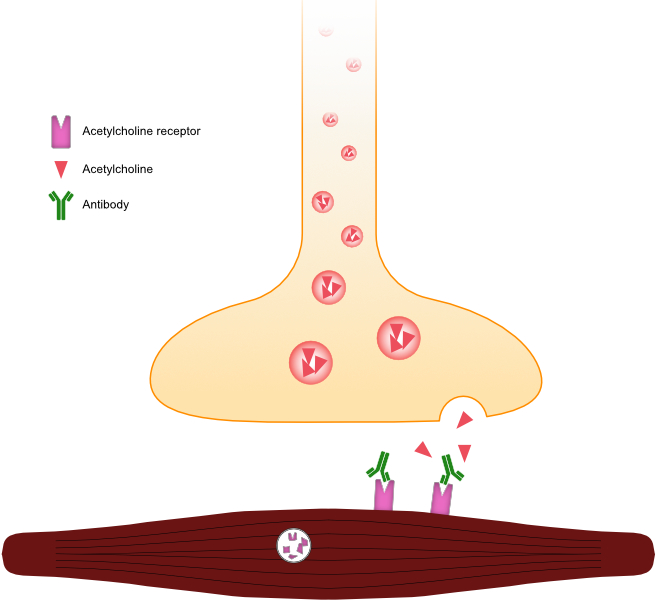
\includegraphics[width=0.5\linewidth]{images/acq-myasthenia} 

}

\caption{Illustration of a motor end plate affected by acquired myasthenia gravis. Note the immunoglobulin binding to the acetylcholine receptor, preventing the binding of acetylcholine, and also leading to endocytosis and decreased receptor density.}\label{fig:acq-myasthenia}
\end{figure}

\chapter{Infectious myositis}\label{infectious-myositis}

\section{Clostridial myositis}\label{clostridial-myositis}

Clostridial infections are \textbf{common and important diseases of
livestock}. Common causes of clostridial disease are \emph{C. septicum},
\emph{C. chauvoei}, \emph{C. perfringens}, \emph{C. novyi}, and \emph{C.
sordellii}. Occasionally more than one species can be cultured. Although
the following conditions are often attributed to specific clostridial
species, these should be considered \emph{the most common cause}, and
not necessarily the \emph{sole} cause. Clostridial disease is caused by
the release of exotoxins, leading to local damage and systemic illness.
They are often fatal.

A common thread in the pathogenesis of clostridial myositis is the
prerequisite for muscle with reduced oxygen tension that leads to
vegetative growth of the organism and the production of damaging
exotoxins. Further detail is found in the sections below.

\subsection{Malignant edema and gas
gangrene}\label{malignant-edema-and-gas-gangrene}

Malignant edema and gas gangrene are two forms of clostridial myositis,
occurring most commonly in the horse but also in cattle and other
livestock. They share a pathogenesis and many clinical signs; it is
simply the presence of gas bubbles that distinguishes gas gangrene from
malignant edema. \emph{C. septicum} is most commonly the cause of
malignant edema, while \emph{C. perfringens} is more frequently isoltaed
from gas gangrene.

Malignant edema/gas gangrene occurs following the introduction of spores
by a deep, penetrating wound, almost always from an injection, though
surgical procedures (castration) may also contribute. Local anaerobic
conditions allow organisms to proliferate and produce exotoxin that
damage blood vessels and myofibers, causing hemorrhage and myonecrosis.
The damage is often extensive and accompanied by a serosanguineous
exudate and extremely foul smell. Microscopically, hemorrhage, edema,
and myonecrosis predominate. Neutrophils and bacteria are present but
are infrequent. Without prompt treatment (antibiotics and fasciotomy,
Figure \ref{fig:fasciotomy}), death occurrs within 24-48 hours.

\begin{figure}

{\centering 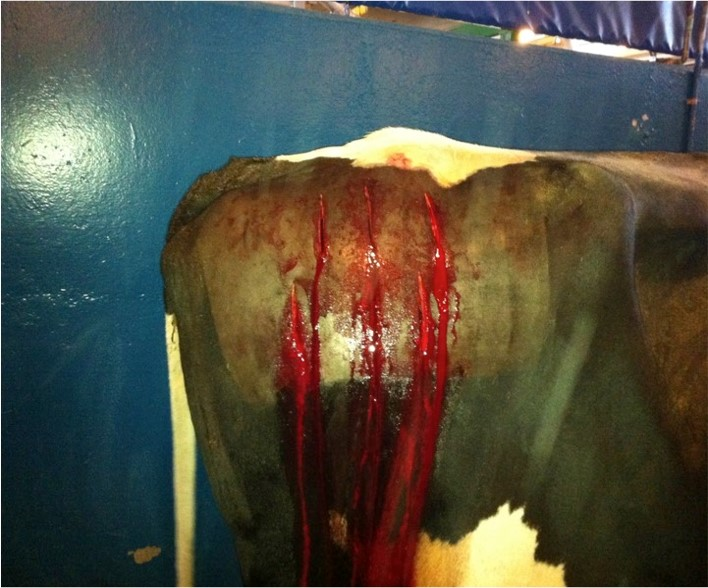
\includegraphics[width=0.6\linewidth]{images/fasciotomy} 

}

\caption{Malignant edema in a cow resulting in marked swelling of the gluteal muscles. This cow was treated with several fasciotomy incisions to release the pressure and allow exposure to oxygen. Image courtesy of Dr. H Staempfli.}\label{fig:fasciotomy}
\end{figure}

\subsection{Blackleg}\label{blackleg}

Blackleg is a \textbf{common and deadly} condition of well-conditioned,
pastured cattle 9 months to 2 years old. The cause of blackleg is
\emph{C. chauveoi}. Unlike malignant edema/gas gangrene,
\textbf{penetrating wounds are not a feature of blackleg}. Instead,
spores are ingested from contaminated pasture, and, through as yet
unknown mechanisms, cross the intestinal mucosa and spread
hematogenously to various organs, including skeletal muscle. \textbf{It
is only when an event creates muscle damage or leads to low muscle
tension} that the disease manifests. Low oxygen tension creates the
right environment for spores to germinate and for organisms to multiply
and release toxin, leading to vascular necrosis, hemorrhage, and
myonecrosis. Lesions are most frequently found in the muscles of the
limbs, though the tongue and diaphragm are also common sites. The
myocardium may also be affected. The clinical course is so rapid that
clinical signs are rarely observed; animals die within 24-36 hours.

The condition derives its name from the gross appearance of muscle at
necropsy, which is typically dark red to black, with or without gas
bubbles. Histologically, severe myonecrosis and fragmentation are
present alongside marked edema and hemorrhage.

\hypertarget{botulism}{\subsection{Botulism}\label{botulism}}

\emph{Note: Botulism and \protect\hyperlink{tetanus}{Tetanus} are
described here, as they are clostridial diseases, but they should be
considered neuromuscular diseases. They do \textbf{NOT} cause a
myositis!}

\emph{C. botulinum} is the causative agent of botulism, a neuromuscular
disease leading to flaccid paralysis of skeletal muscle. Horses are
particularly susceptibe. In foals \textless{} 6 months of age, ingestion
of \emph{C. botulinum} spores can lead to proliferation of the organism
and production of botulinum toxin. In adult horses, it is more commonly
the ingestion of botulinum toxin, not the bacteria itself, that is the
cause of the disease. Hay contaminated with the corpses of rodents is a
common source of botulinum toxin. Botulinum toxin spreads hematogenously
to the neuromuscular junction where it is taken up by the terminal axon.
Botulinum toxin binds to synpatic vesicles containing acetylcholine,
preventing their release, and thereby preventing the spread of action
potentials, ultimately resulting in paralysis. There are no gross or
histological lesions.

\hypertarget{tetanus}{\subsection{Tetanus}\label{tetanus}}

Like \protect\hyperlink{botulism}{Botulism}, tetanus is the result of a
clostridial toxin affecting neurotransmitter release. It develops when
spores of \emph{C. tetani} are introduced into tissue by penetrating
injuries. Anaerobic conditions at the site of injury prompt the spores
to vegetate. Tetanus toxin is taken up by endocytosis into the axon of
the nearest motor neuron and brought via retrograde transport to the
neuronal cell body within the spinal cord. There the tetanus toxis is
released, and is then taken up by the axon of an \emph{inhibitory}
neuron. Once within the inhibitory neuron, the toxin acts in a fashion
similar to that of botulinum toxin, and interferes with the release of
acetylcholine. \emph{It is the abolishment of inhibitory signals that
leads to the clinical signs associated with tetanus}. Motor neurons are
under more or less constant stimulation, and the inhibitory neurons
serve to counter balance this stimulation. With the removal of
inhibitory constraint, all that is left is stimulation, leading to
prolonged, severe muscle contraction.

Horses, guinae pigs, and humans are most susceptible to disease, while
dogs and cats are relatively resistant. There are no gross or histologic
lesions.

\hypertarget{suppurative-myositis}{\section{Suppurative
myositis}\label{suppurative-myositis}}

Suppurative myositis is most commonly the result of innoculation from
trauma or surgery. Occasionally, abscesses can develop in muscle through
extension from nearby structures (e.g.~joint or tendons), or through
hematogenous spread. The most common bacterial isolates from muscle
abscesses are given in Table \ref{tab:abscess}.

\begin{table}[t]

\caption{\label{tab:abscess}Most common bacterial isolates from muscle abscesses in veterinary species}
\centering
\begin{tabular}{>{\raggedright\arraybackslash}p{15em}>{\em\raggedright\arraybackslash}p{15em}}
\toprule
Species & Bacteria\\
\midrule
Cattle & T. pyogenes\\
Swine & C. pseudotuberculosis, H. parasuis\\
Sheep & C. pseudotuberculosis\\
Goats & C. pseudotuberculosis\\
Horses & C. pseudotuberculosis, S. equi\\
\addlinespace
Cats & P. multocida\\
\bottomrule
\end{tabular}
\end{table}

\chapter{Neoplasms of muscle}\label{neoplasms-of-muscle}

Primary neoplasms of the striated muscle are rare in veterinary species.
Although usually found in muscle, they can arise in unexpected locations
devoid of striated muscle, such as the bladder.

\section{Rhabdomyoma}\label{rhabdomyoma}

As it's name suggests, a rhabdomyoma is a benign tumour of striated
muscle. It is seen most frequently in the hearts of pigs, particularly
the red wattle breed. They are typically incidental findings. They
present grossly as circumscribed, smooth-surfaced, nodular masses
embedded in the myocardium. A similar neoplasm occasionally arises on
the larynx of dogs. Laryngeal rhadomyomas may cause respiratory
difficulty or altered bark. They are typically minimally invasive and
tend not to metastasize.

\section{Rhabdomyosarcoma}\label{rhabdomyosarcoma}

These are the malignant counterparts to rhadomyomas. They are most
common in the dog. Counterintuitively, they occur more frequently at
sites that normally lack skeletal muscle versus those that don't. There
are a variety of subtypes, however, whether there is any prognostic
significance to differentiating them is uncertain. They all tend to be
locally invasive and metastatic. Prognosis is poor for all subtypes.
Grossly, the tumours appear as pale, white to tan, firm masses, often
with areas of necrosis. The botryoid (``cluster of grapes'') subtype
occurs in the bladder as a polypoid mass. The histologic appearance of
these tumours is quite variable, though occasionally elongated, variably
striated, myotube-like cells known as ``strap cells'' are present, which
is suggestive of rhadomyosarcoma. Immunohistochemistry is usually
required to definitively diagnose these tumours.

\section{Non-muscle primary tumours of
muscle}\label{non-muscle-primary-tumours-of-muscle}

Granular cell tumours occur in the tongue of dogs and cats. They are
composed of densely packed round cells with PAS positive granules. The
supporting mesenchyme of muscle can occasionally produce a (usually)
malignant neoplasm. Hemangiosarcomas can arise in the muscles of dogs
and horses, and aspiration of these large, intramuscular masses
typically only reveals hemorrhage. Like their splenic cousins, they
metastasize frequently.

\section{Secondary tumours}\label{secondary-tumours}

Muscles are occasionally infiltrated by local neoplasms. Infiltrative
lipomas are characterized by relatively well differentiated adipocytes
crawling and invading through myofibers. They are highly invasive and
require excision. Other neoplasms, such as subcutaneous mast cell
tumours, lymphoma, hemangiosarcomas, and soft tissue sarcomas can invade
into muscle. Metastasis to muscle is uncommon but does occur.

\chapter{Parasitic myositis}\label{parasitic-myositis}

Parasitic diseases of the muscle are rarely pathological to the host,
but are a critical part of the lifecycle of several important parasites.
Generally speaking, the most important aspect of parasitic diseases of
muscles in animals is their threat to human health.

\hypertarget{sarcocystosis}{\section{Sarcocystosis}\label{sarcocystosis}}

Sarcocysts are a very common protozoan parasite found in the muscle of
herbivores. They have an in indirect life cycle. Carnivores are
typically the definitive host, and become infected through consumption
of muscle from an infected intermediate host. Most herbivorous species
have their own \emph{Sarcocystis} species (e.g. \emph{S. bertrami} in
horses, \emph{S. cruzi} in cattle, and \emph{S. tenella} in sheep), and
sarcocysts are routinely found in the muscles of theses species, almost
always with little to no associated pathology. Rarely, pathology in the
form of myositis can occur. Even less commonly, cattle and sheep may
develop eosinophilic myositis, which is thought to be caused by the
degeneration of sarcocysts and which provokes a profound -- and deadly
-- eosinophilic myositis. This grossly presents as distinctive, well
demarcated areas of green discolouration the muscle.

\section{\texorpdfstring{\emph{Neospora caninum} and \emph{Toxoplasma
gondii}}{Neospora caninum and Toxoplasma gondii}}\label{neospora-caninum-and-toxoplasma-gondii}

Although more commonly associated with abortion and neurological
disease, \emph{N. caninum} and \emph{T. gondii} both occasionally
present as a disease of muscle. Puppies and kittens tends to be affected
most often. The disease manifests as a myositis with lymphoplasmacytic
inflammation, myonecrosis, and atrophy.

\section{Trichinellosis}\label{trichinellosis}

\textbf{Trichinellosis is an important parasitic disease of animals and
humans}. Several species of \emph{Trichinella} exist. The most common is
\emph{T. spiralis}. The parasite infects a multitude of species,
including pigs, dogs, cats, bears, rodents, and many other wild animals.
The disease in humans in North America has largely become historical due
to routine meat inspection, but does still affect people, and is still
present in wild carnivores. Wild animals of the arctic, such as walrus
and polar bears, are an important source of food for the Inuit, and
represent a particularly important risk of Trichinella. Ingestion of
undercooked wild meat is perhaps the most important risk factor for
human trichinellosis.

The life cycle of \emph{Trichinella} spp. is relatively simple. Nematode
larva encysted in muscle are consumed, and released by the gastric
juices of the host. The liberated larva molt into adults and reproduce.
The females the penetrate through the intestinal crypts (the males die),
and deposit larva into the lymphatics. The larva travel through the
lymphatic system and into the systemic circulation, where they then
preferentially encyst into muscles, and await the next cycle. Those that
do not encyst in muscle are cleared by the immune system. Through an
unknown mechanism, the larva encyst prefentially in the
\textbf{diaphragm, tongue, laryngeal muscles, and masseter muscles}.

The pathology caused by \emph{Trichinella} spp. is relatively mild. A
single larva will enter into a single myofiber, where it enlarges and
coils. The myofiber undergoes some changes, including enlargement of the
nuclei, decrease in number of myofibrils, and an increase in the
thickness of the basal lamina, to become what is known as a ``nurse
cell''. Rarely, lymphoplasmacytic inflammation is present. Larva can
live in an encysted form for over 20 years, and \emph{T. nativa}, the
species found in northern animals, resists freezing.

Trichinellosis is zoonotic. In humans, clinical signs and symptosm
related to trichinellosis include fever, myalgia, facial edema, rash,
and occasionally chronic diarrhea.

\section{Cysticercosis}\label{cysticercosis}

The taxonomy and nomenclature of the tapeworms is confusing and
frustrating. Adult taenids are classified separately from their
intermediate form, the cysticerci. \emph{Cysticercosis is the result of
consumption of teanid eggs, not the consumption of cysticerci.} It is
the pathology related to the development of cysticerci in the muscle,
and is still an important disease in developing countries.

Like many parasites, the life cycle of tapeworms revolves around a
predator-prey dynamic. Predators are the definitive host of the adult
tapeworm and are infected through consumption of larval stages in the
flesh of the prey. Larva of tapeworms go through several developmental
cycles, one of which is a cysticercus, in the intermediate host. In some
tapeworm species, the cysticercus has a predilection site for skeletal
muscle; it is those species that interest us here, and which are
described in Table \ref{tab:cysti}.

\begin{table}[t]

\caption{\label{tab:cysti}Tapeworm and cysticercus species, along with their hosts and predilection sites}
\centering
\begin{tabular}{>{\em\raggedright\arraybackslash}p{5em}>{\raggedright\arraybackslash}p{10em}>{\em\raggedright\arraybackslash}p{7em}>{\raggedright\arraybackslash}p{6em}l}
\toprule
Tapeworm & Definitive.host & Cysticercus & Intermediate.host & Predilection.site\\
\midrule
T. solium & Human & C. cellulosae & Pigs (and humans) & Heart, masseter, tongue\\
T. saginata & Human & C. bovis & Cattle & Heart, masticatory muscles\\
T. ovis & Dogs, wild carnivores & C. ovis & Sheep and goats & Heart, skeletal muscle\\
\bottomrule
\end{tabular}
\end{table}

The pathology in intermediate hosts is fairly minimal. Cysticerci form
grossly visible cysts (1-2 cm) containing clear fluid and a larva. These
may elicit a mild lymphoplasmacytic and eosinophilic inflammatory
response, but otherwise do not harm the host. Dead larva become heavily
calcified.

Occasionally, cysticerci can infect in an unusual intermediate host and
form cysts in devastating anatomic locations. Consider the life cycle of
\emph{T.solium} and \emph{C. cellulosae}. Adult tapeworms living in the
definitive host, humans, pass eggs or proglottids in their feces, which
are normally taken up by pigs, in which cysticerci form in muscle.
Occasionally, however, humans can \emph{also} come ingest the eggs, in
which case the cysticerci develop not just in muscle, but also in brain
and eyes, with devastating consequence. This condition can be
devastating and is still prevalent in areas of high poverty and poor
sanitation.

\bibliography{book.bib,packages.bib}


\end{document}
